\chapter{Stability Problem of DC Source}

\section{The Bridge Rectifier}

\begin{figure}[H]
  \centering
  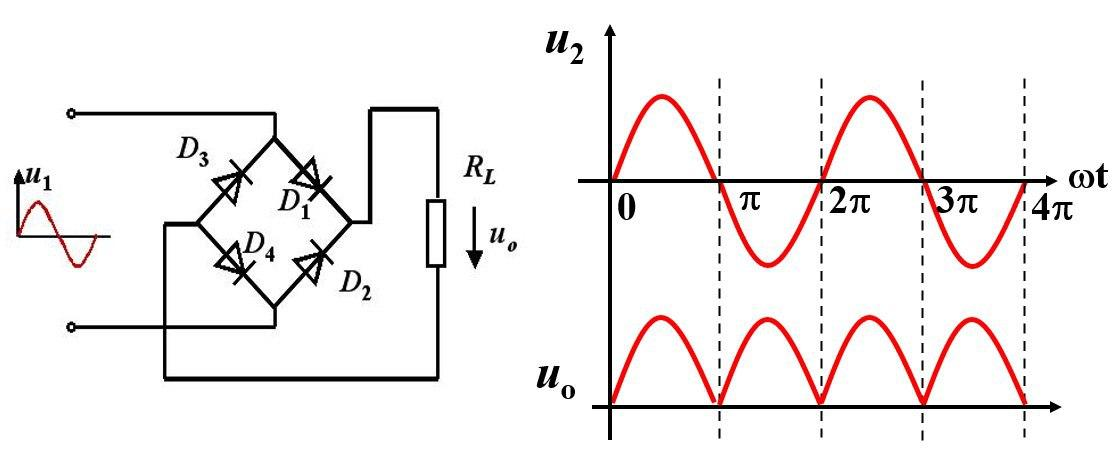
\includegraphics[width=0.9\linewidth]{figures/BridgedRectifierCircuit}
  \caption{A Bridged Rectifier Circuit}
\end{figure}

\begin{equation*}
  \begin{aligned}
    V_L \approx 0.9 V_S \quad\quad \quad\quad \quad\quad \quad\quad  I_{DI} = I_{D2} = I_{D3} = I_{D4} = \dfrac{0.45 V_S}{R_L} 
  \end{aligned}
\end{equation*}

\section{Filter}

\begin{figure}[H]
  \centering
  \begin{subfigure}{.5\textwidth}
    \centering
    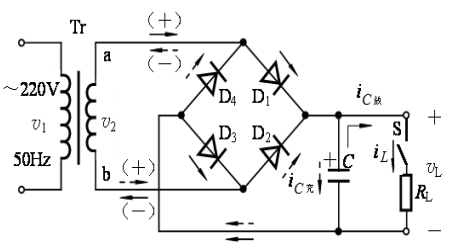
\includegraphics[width=\linewidth]{figures/Filter-1}
  \end{subfigure}
  \begin{subfigure}{.45\textwidth}
    \centering
    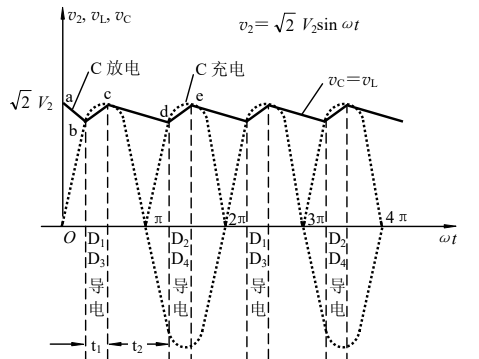
\includegraphics[width=\linewidth]{figures/Filter-2}
  \end{subfigure}
\end{figure}

\section{Series Feedback Voltage Regulator}

\begin{figure}[H]
  \centering
  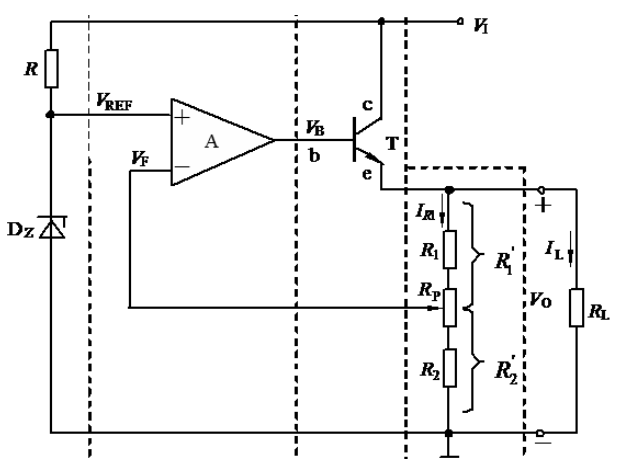
\includegraphics[width=\linewidth]{figures/Series-Feedback-Voltage-Regulator}
\end{figure}

\begin{equation*}
  \begin{aligned}
    V_O = V_{REF} \left( 1 + \dfrac{R_1}{R_2}  \right)
  \end{aligned}
\end{equation*}

\section{Integrated Voltage Regulator}

\begin{figure}[H]
  \centering
  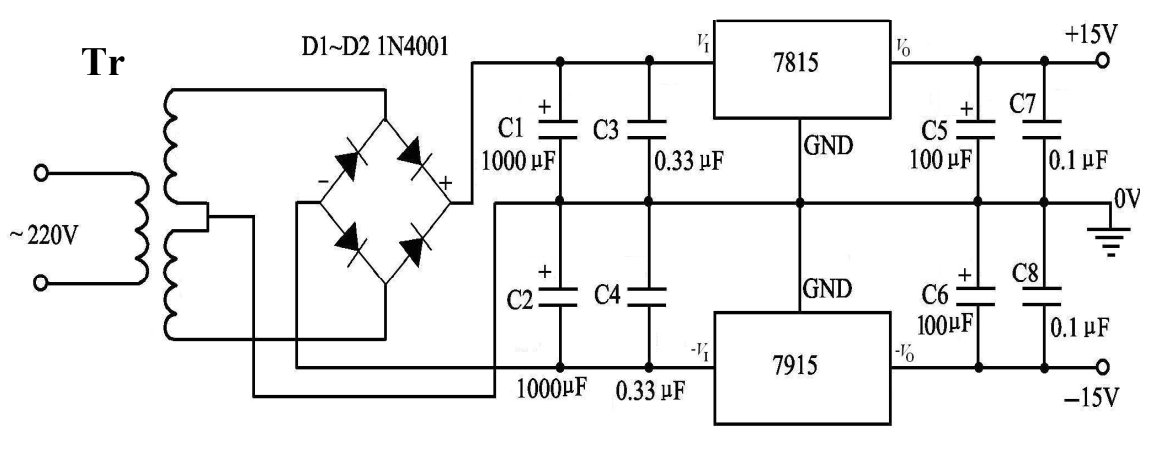
\includegraphics[width=\linewidth]{figures/Integrated-Voltage-Regulator}
\end{figure}

%%% Local Variables:
%%% mode: latex
%%% TeX-master: "Analogue_Electronics"
%%% End:
